\chapter{Results and Discussion}
The device has been designed completely from scratch. So, to make it standard compliant it is necessary to test all its aspect and keep them well below the limit so that final results are well within the stipulated guideline. Hence, here qualitative and quantitative results are presented which include computation latency, reporting rate \& variation, ADC response(s) and amplitude \& frequency estimation.

\section{Frequency Computation}
\subsection{Steady State Nominal Frequency Operation}
First, we will see the frequency response of the device. First nominal frequency test was done, where device was given 50 Hz nominal frequency.
\begin{figure}[h]
	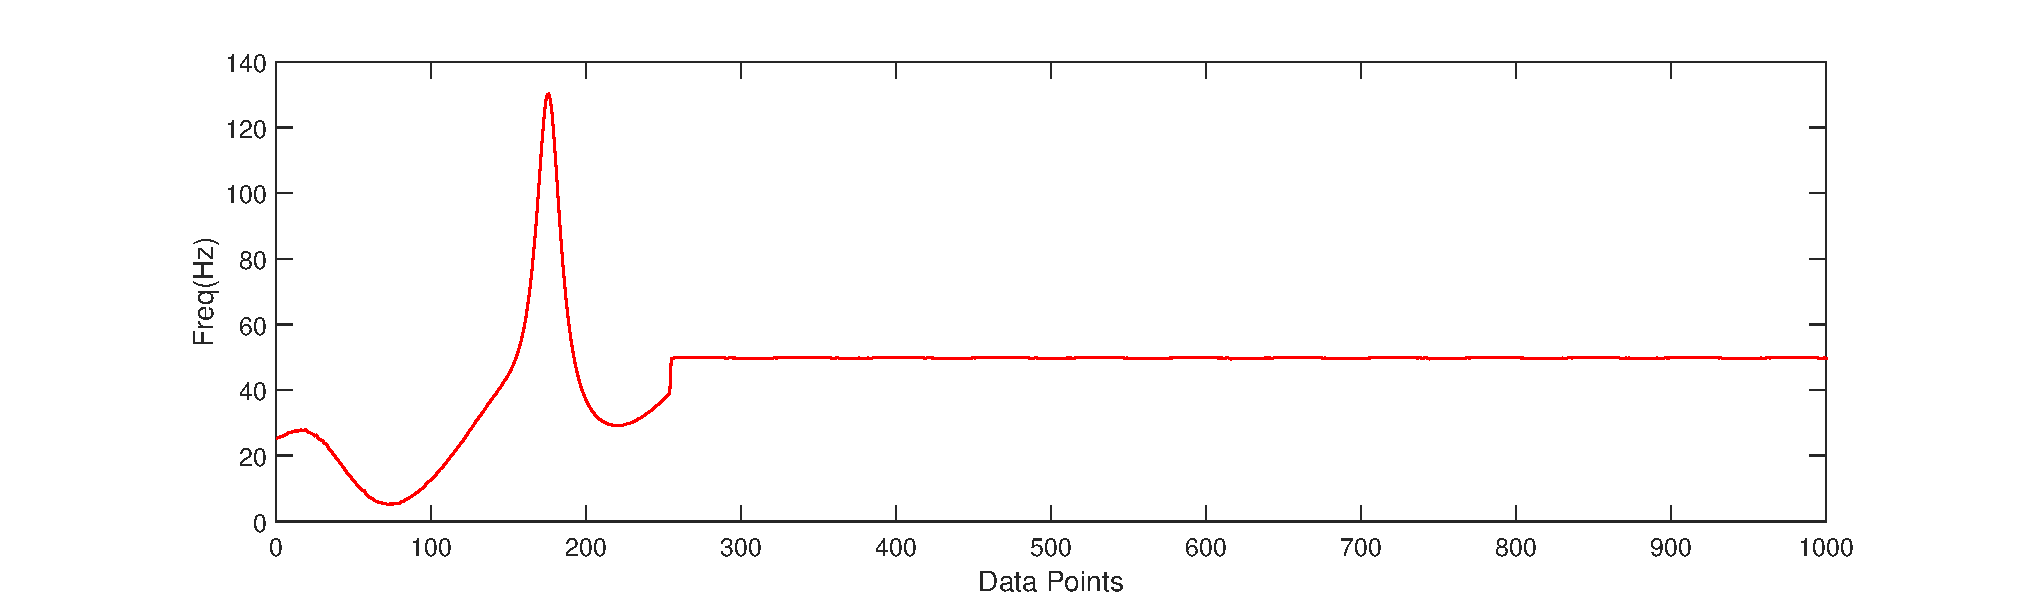
\includegraphics[width=\textwidth]{fig/50Hz_freq_1000samples.eps}
	\caption{Deice Frequency Response to 50 Hz sine input}
	\label{fig:50hzlongdata}
\end{figure}

In Fig: \ref{fig:50hzlongdata} shows response to an input signal of fundamental frequency 50 Hz. As it can be seen the initial portion has irregularities because of the moving window not being completely filled. length of moving window is 256 samples, hence for first two cycles the window is filled with zeros, which slowly gets filled and then device settles to a final steady state position.

\begin{figure}[h]
	\includegraphics[width=\textwidth]{fig/50Hz_freq_closeup.eps}
	\caption{Zoom-in plot of steady state frequency reading}
	\label{fig:50Hzcloseup}
\end{figure}


If the end part (i.e. steady state, for the device) is zoomed in then oscillation and noise can be seen in the reading as show in Fig: \ref{fig:50Hzcloseup}. It is important to note here, that the plot shown here are instantaneous frequency given by the device, as a qualitative representation of each DFT computation at each point on wave, instead of the averaged value over a cycle. Error was computed on non-averaged instantaneous values and following results weere obtained as show in Fig: \ref{fig:50Hz error}.

\begin{figure}[h]
	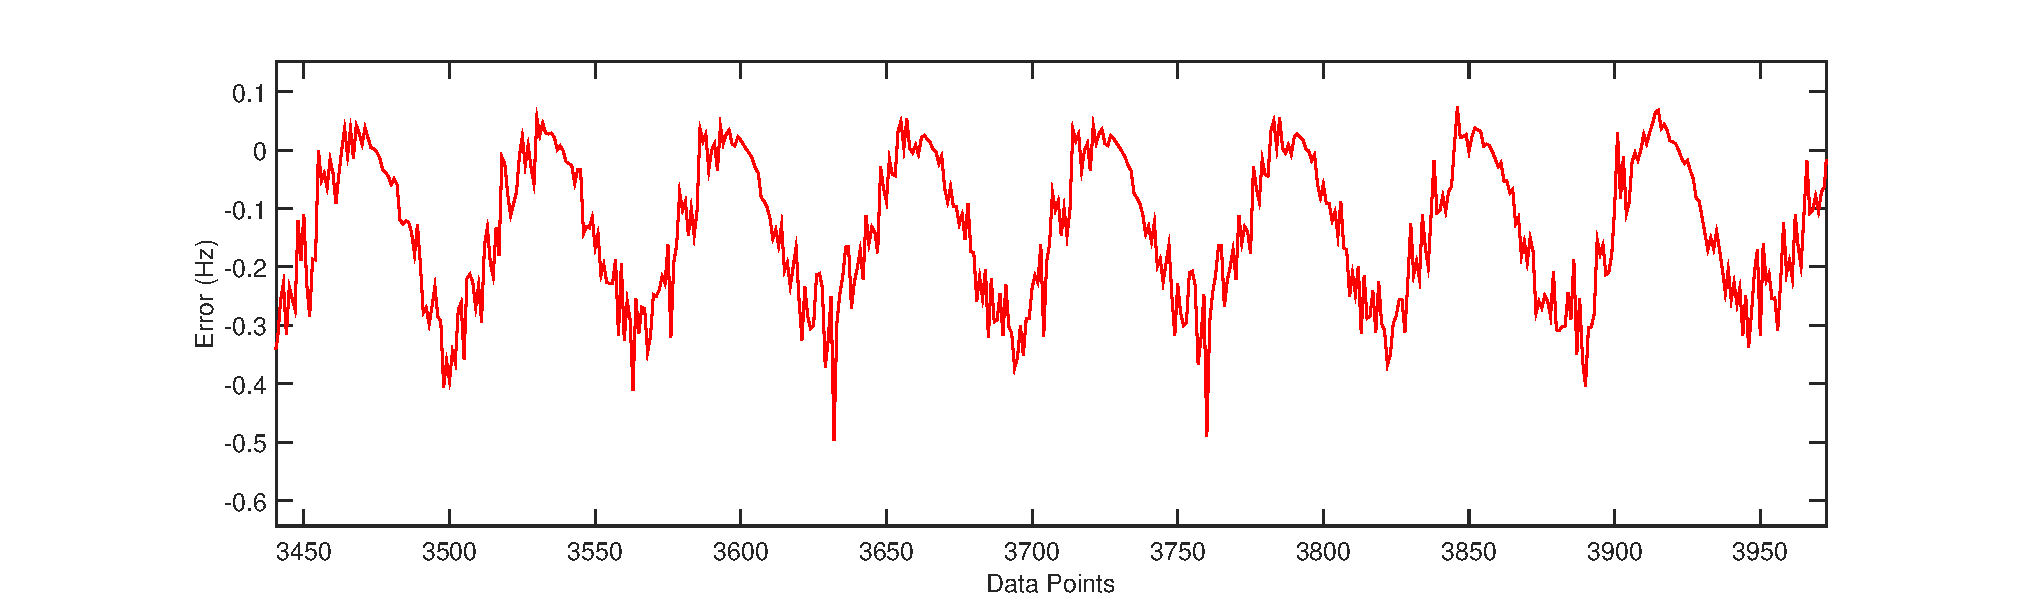
\includegraphics[width=\textwidth]{fig/50Hz_freq_error_closeup.eps}
	\caption{Error Plot for 50 Hz input}
	\label{fig:50Hz error}
\end{figure}
For verifying the results coming from the developed PMU, a simulation program was written, same 256 sample moving window DFT was implemented and same nominal frequency input was given which resulted in to output which is show in Fig: \ref{fig:50Hz simulation}. It is important to note here that though by appearance simulation result \emph{profile} looks worse than the actual results obtained from hardware but in reality they are not, it is due to the the high degree of precision. Here as it can be seen in Fig: \ref{fig:50Hz simulation} range of values is  \texttt{Max:49.99999999995302} to \texttt{Min: 50.00000000005302}, which can practically be considered 50.0 Hz. 
\begin{figure}[h]
	\includegraphics[width=\textwidth]{fig/50Hz_simulated.eps}
	\caption{Simulation Output at 50 Hz}
	\label{fig:50Hz simulation}
\end{figure}
   
\subsection{Steady State Off-nominal Frequency Behaviour}
Qualitatively ability to compute/detect the off-nominal frequency effectively is an important factor. So here different frequency values (i) 50.2 Hz (ii) 50.5 Hz (iii) 49.8 Hz \& (iv) 49.5 Hz are considered for evaluation of device. 

\subsubsection{49.5 Hz Operation}
\begin{figure}[h]
	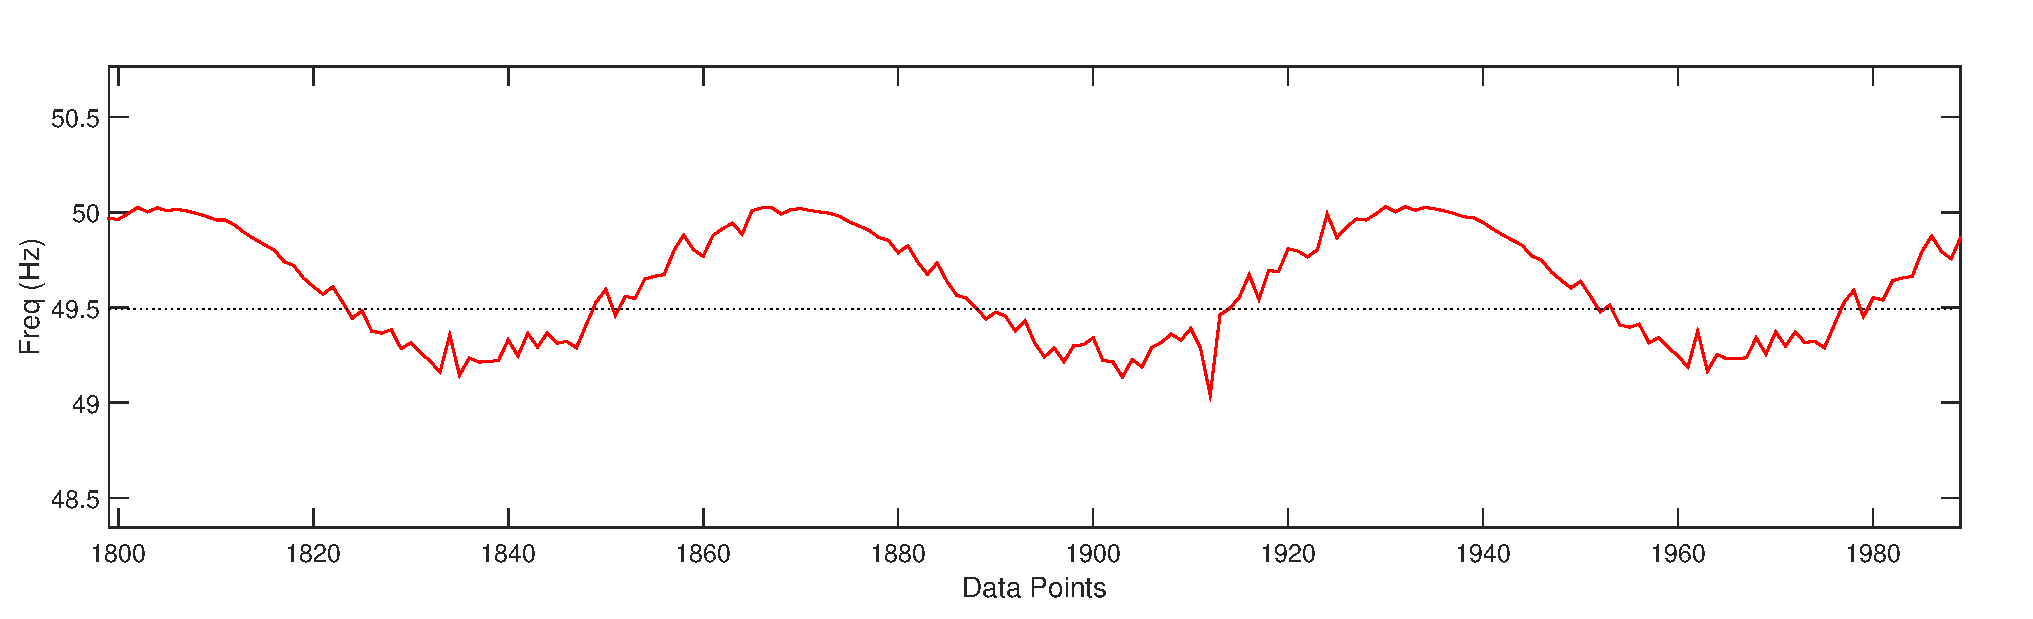
\includegraphics[width=\textwidth]{fig/495Hz_freq_reading.eps}
	\caption{Device reading at 49.5 Hz}
	\label{fig:49.5Hz operation}
\end{figure}
For the off-nominal frequency operation a guide line is drawn on the plot and as it can be seen, that PMU follows perfectly the marker. This is raw data if it is averaged out then it would accurately report the input wave frequency.Range of readings was \texttt{Max:50.12} to \texttt{Min:48.807} Hz

\subsubsection{49.8 Hz Operation}
\begin{figure}[h]
	\includegraphics[width=\textwidth]{fig/498Hz_freq.eps}
	\caption{Device reading at 49.8 Hz}
	\label{fig:49.8Hz operation}
\end{figure}
Fig: \ref{fig:49.8Hz operation} show the operation of PMU at 49.8 Hz input signal. It can be observed that the operation is quiet poor on off-nominal frequency.

\subsubsection{50.2 Hz Operation}
\begin{figure}[h]
	\includegraphics[width=\textwidth]{fig/502_Hz_freq.eps}
	\caption{Device Reading at 50.2 Hz}
	\label{fig:50.2Hz operation}
\end{figure}
As it can be seen in Fig: \ref{fig:50.2Hz operation} PMU was giving poorer responses. Overall average frequency reported was 50.05 Hz with samples varying in range of \texttt{Max:50.35 Hz} to \texttt{Min:49.99 Hz}.


\subsubsection{50.5 Hz Operation}
\begin{figure}[h]
	\includegraphics[width=\textwidth]{fig/505_Hz_freq.eps}
	\caption{Device reading at 50.5 Hz}
	\label{fig:50.5Hz operation}
\end{figure}
Comparison of Fig: \ref{fig:50.5Hz operation} with previous figures, like Fig: \ref{fig:50.2Hz operation}, Fig: \ref{fig:49.8Hz operation} and Fig: \ref{fig:49.5Hz operation} it can be clearly observed that there is a deterioration in the profile and it is well drifted away from the standard result.The deviation observed was \texttt{Max:50.23 Hz} to \texttt{Min:50.16 Hz}.
%%
%\subsection{Error Plot}
%A plot of error existing in the each test case is plotted to give an overview of %error(s) in the result(s).  

%===========================================================================

\section{Phase Computation}
\subsection{Steady State Nominal Frequency Phase results}
 
\begin{figure}[h]
	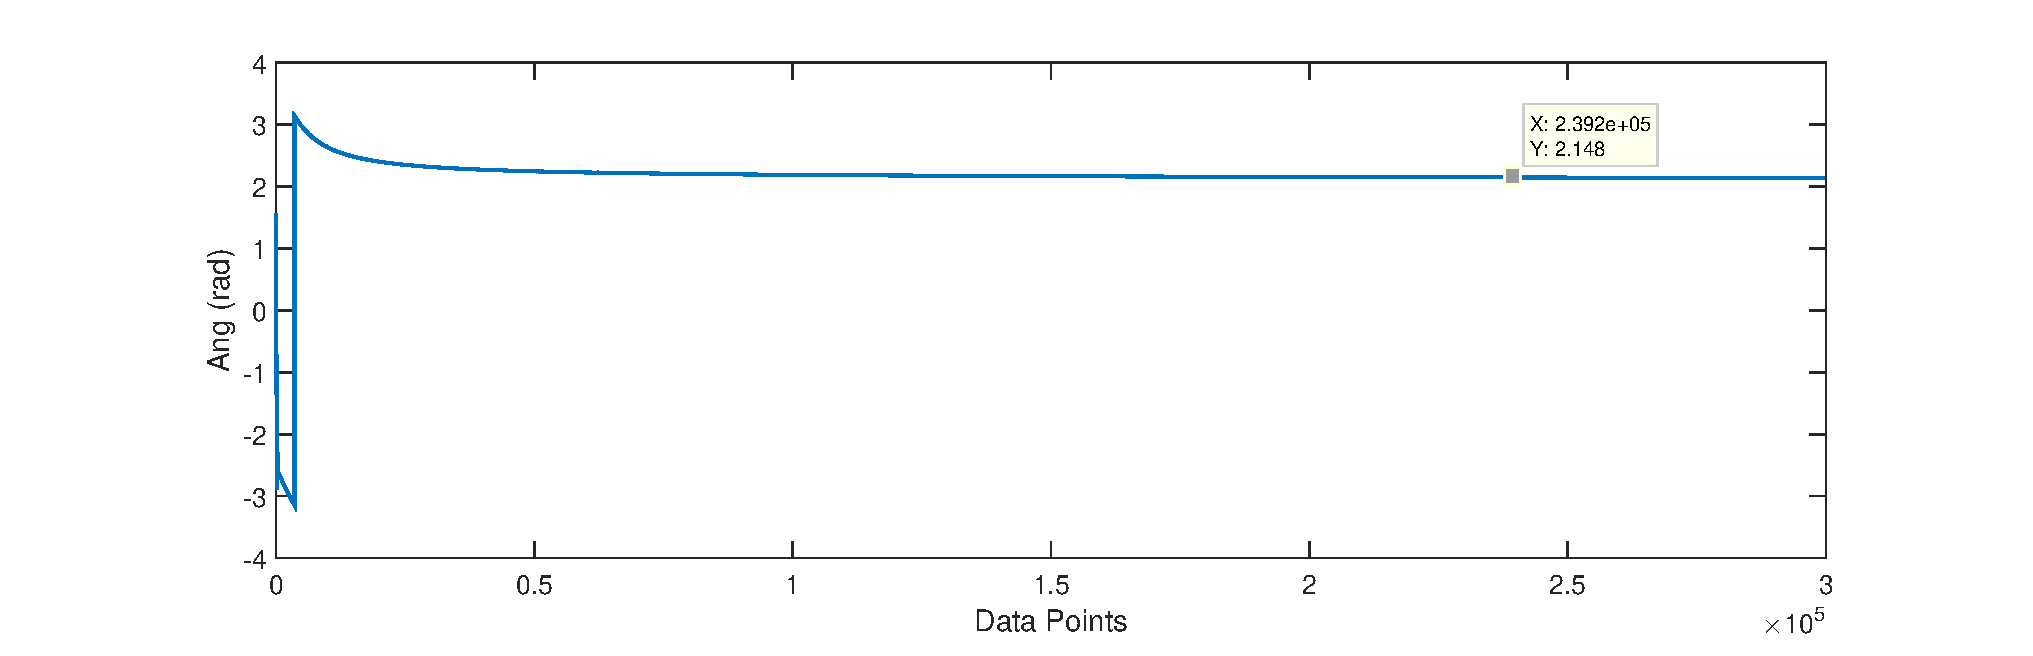
\includegraphics[width=\textwidth]{fig/50Hz_angle.eps}
	\caption{Phase angle at 50 Hz}
	\label{fig:50Hz ang}
\end{figure}
Fig: \ref{fig:50Hz ang} shows the phase reported by the device for a 50Hz input signal. And as expected it settles to a steady state value this proves that there exist zero relative angular velocity between the reference frame and the input signal. Now we will see angle reporting performance for other few frequencies.

\subsection{Steady State Off-nominal Frequency Phase results}
Contrary to the steady state 50 Hz operation, in case of off nominal frequency operation the angle of phasor keeps changing (due to the leakage effect) either increasing or decreasing depending upon the relative frequency). 
\subsubsection{49.5 Hz Operation}
\begin{figure}[h]
	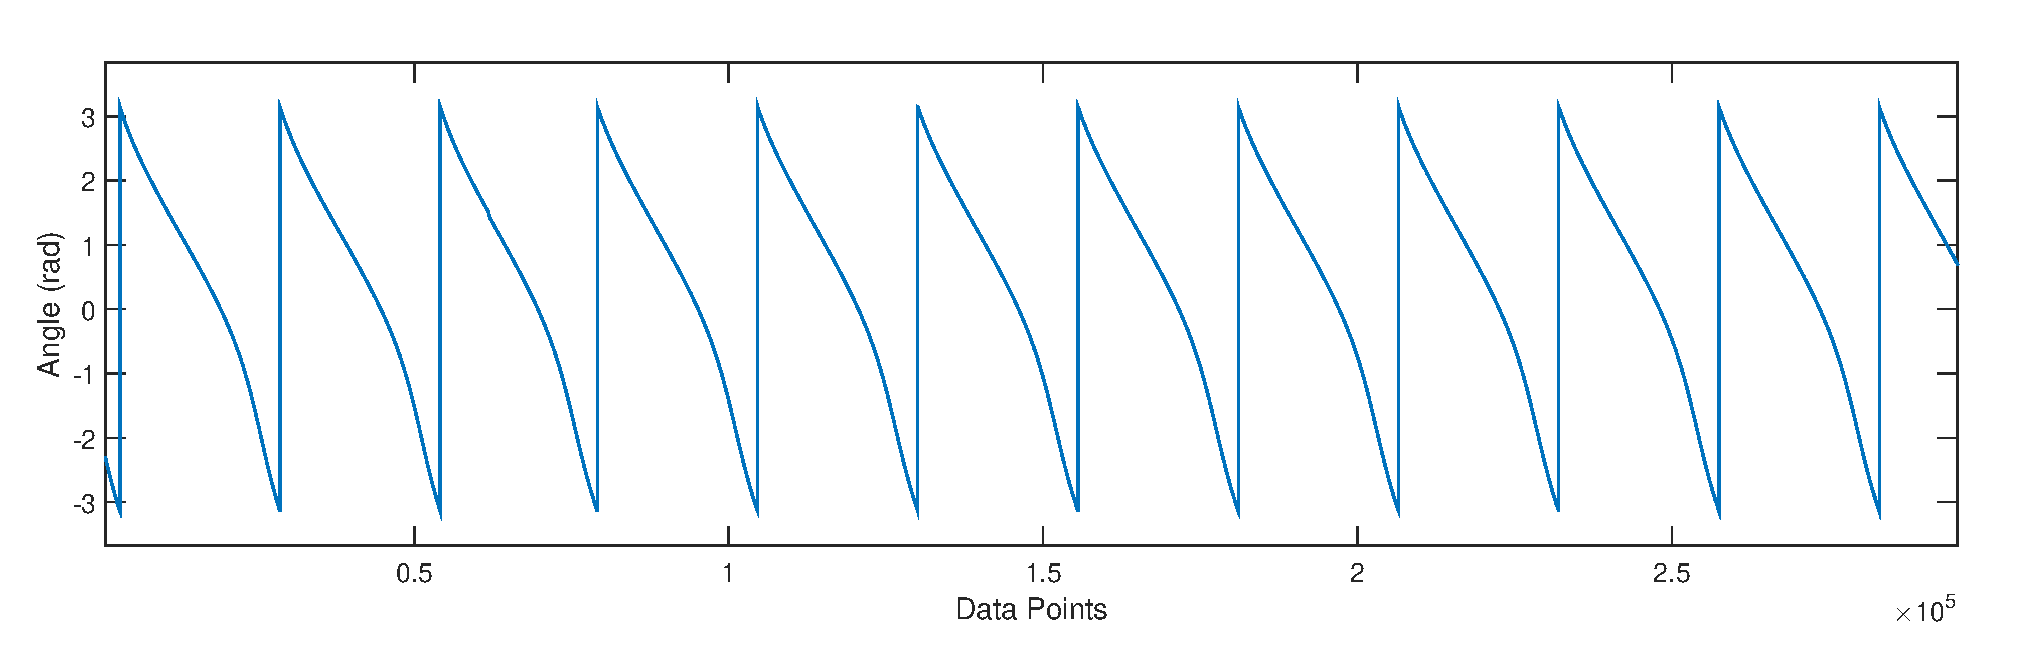
\includegraphics[width=\textwidth]{fig/495Hz_ang.eps}
	\caption{Phase angle of 49.5 Hz input signal}
	\label{fig:49.5Hz ang}
\end{figure}

\begin{figure}[h]
	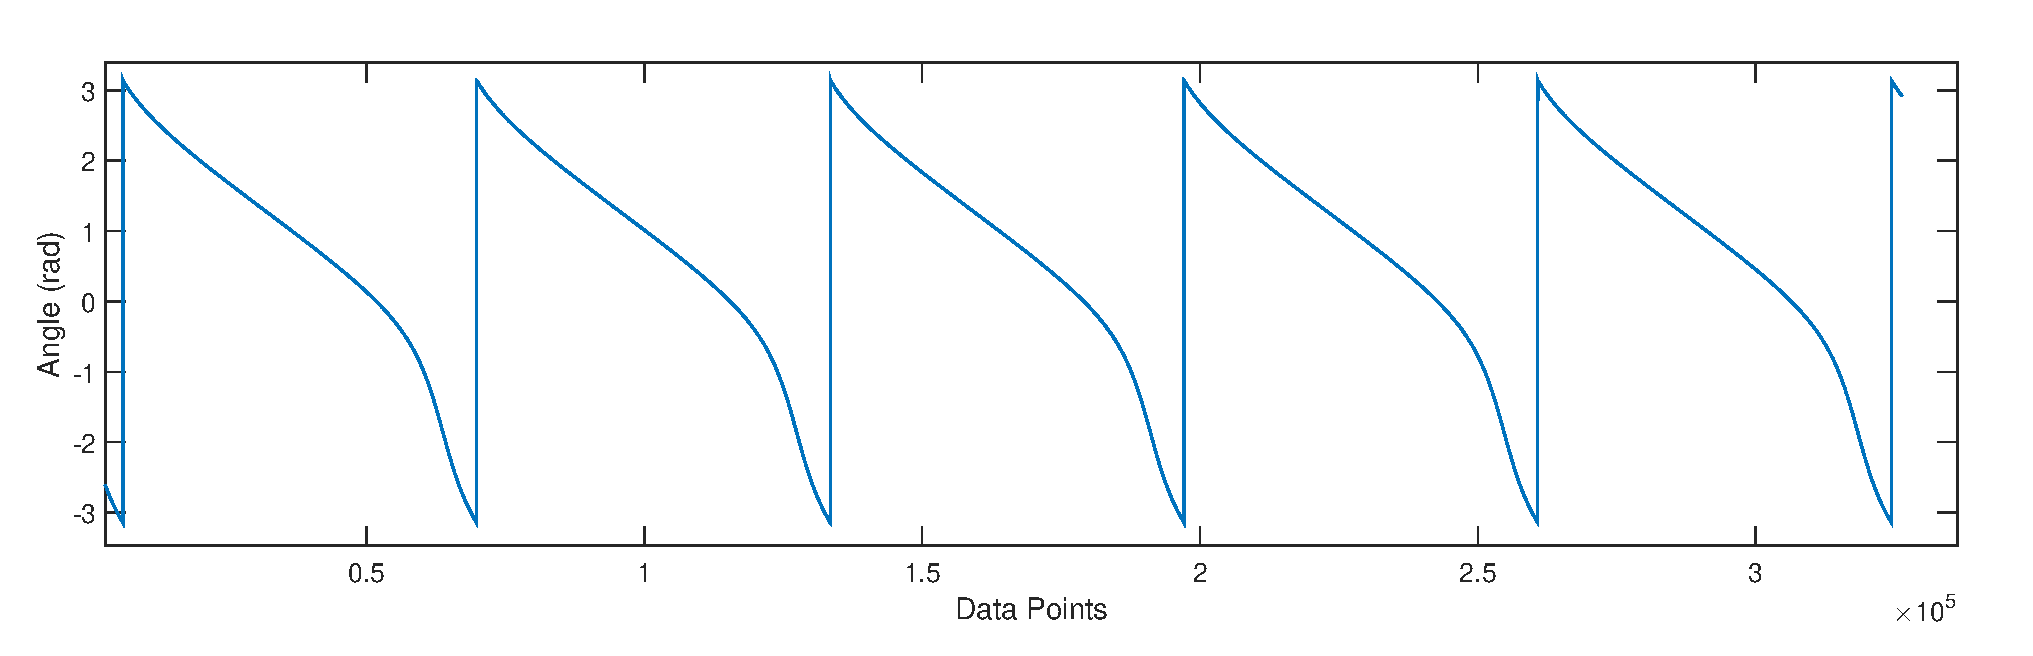
\includegraphics[width=\textwidth]{fig/498Hz_ang.eps}
	\caption{Phase angle of 49.8 Hz input signal}
	\label{fig:49.8Hz ang}
\end{figure}
 
Representative plots of two phasors at 49.5 Hz and 49.8 Hz are presented here. And we can see the \emph{angle wrap} taking place due to relative difference in angular velocity.

\subsubsection{Computation delay}
Completion of all computation and processing within given time limit is necessary. For 50 Hz system 20 ms is the time period within which whole process should be over. In this section we will see the latency involved in computation. Fig: \ref{fig:simpleLatency} shows the time taken by the program in computing DFT.

\begin{figure}[h]
	\includegraphics[width=\textwidth]{fig/simple_latency.eps}
	\caption{Normal computation latency}
	\label{fig:simpleLatency}
\end{figure}

As it can be seen from Fig: \ref{fig:simpleLatency}, time taken by the program is way below the threshold. There are peaks seen in-between, which are caused partly because of other OS services running in background and partly due to the C-program copying the new data from the PRU buffer to the RAM.   

\begin{figure}[h]
	\includegraphics[width=\textwidth]{fig/optimised_latency.eps}
	\caption{Compiler optimised latency}
	\label{fig:optimisedLatency}
\end{figure}
Fig: \ref{fig:optimisedLatency} shows latency of the DFT computation after compilation time optimization. Details about the runtime optimization and compilation optimizations are given in Appendix-B.

